\subsection*{Aufgabe 11}
Die folgende approximierende Verteilungsfunktion beschreibt die Verteilung des Merkmals
"Alter" in der aktuellen Gesamtheit aller Mitglieder des Kreisverbands einer Partei. Zur
Bestimmung dieser Verteilungsfunktion wurde das Merkmal in sechs Klassen eingeteilt.

\begin{center}
\begin{figure}[!htbp]
\fbox{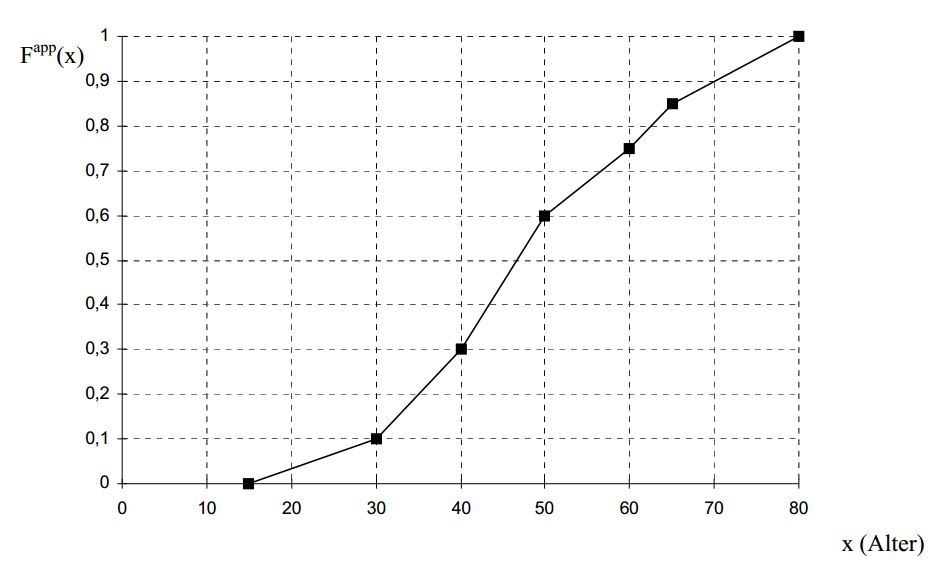
\includegraphics[width=0.9\textwidth,page=1]{chapters_AB/Grafiken_AB/AB_1_11.jpg}} \caption{Erkl�rung}
\end{figure}
\end{center}

\begin{enumerate} [label=\alph*)]
\item Geben Sie die Klassengrenzen und die jeweiligen relativen H�ufigkeiten innerhalb der
Klassen an!
\item Bestimmen Sie approximativ anhand der Grafik (keine Rechnung n�tig!) den Median
dieser Verteilung!
\item Welcher (approximative) Anteil der Parteimitglieder ist 70 Jahre oder �lter? (Keine
Rechnung n�tig!)
\end{enumerate}



